\documentclass[12pt]{article}
\usepackage{amsmath}
\usepackage{amssymb,float}
\usepackage{graphicx}
\usepackage{subcaption}
\usepackage{hyperref}
\usepackage{flexisym}
\usepackage{color}
\usepackage{breqn}
\usepackage{rotating}
\usepackage{tikz}
\usepackage[utf8]{inputenc}
\usepackage{tabularx, blkarray}
\usepackage[linesnumbered,boxed]{algorithm2e}
\newcommand\colhead[1]{\multicolumn{1}{>{$}c<{$}}{#1}}
\usepackage{eqparbox}
\usepackage{listings}
\definecolor{mygreen}{RGB}{28,172,0} % color values Red, Green, Blue
\definecolor{mylilas}{RGB}{170,55,241}
\lstset{language=Matlab,%
    %basicstyle=\color{red},
    breaklines=true,%
    morekeywords={matlab2tikz},
    keywordstyle=\color{blue},%
    morekeywords=[2]{1}, keywordstyle=[2]{\color{black}},
    identifierstyle=\color{black},%
    stringstyle=\color{mylilas},
    commentstyle=\color{mygreen},%
    showstringspaces=false,%without this there will be a symbol in the places where there is a space
    numbers=left,%
    numberstyle={\tiny \color{black}},% size of the numbers
    numbersep=9pt, % this defines how far the numbers are from the text
    emph=[1]{for,end,break},emphstyle=[1]\color{red}, %some words to emphasise
    %emph=[2]{word1,word2}, emphstyle=[2]{style},    
}
\newcommand*{\captionsource}[2]{%
  \caption[{#1}]{%
    #1%
    \\\hspace{\linewidth}%
    \textbf{Source:} #2%
  }%
}

\newcommand{\Rea}{{\Bbb R}}
\newcommand{\Int}{{\Bbb Z}}
\newcommand{\Rat}{{\Bbb Q}}
\newcommand{\Cmp}{{\Bbb C}}
\newcommand{\Nat}{{\Bbb N}}

\setlength{\oddsidemargin}{.25in} \setlength{\evensidemargin}{.25in}
\setlength{\textwidth}{6in} \setlength{\topmargin}{0.0in}
\setlength{\textheight}{8.5in}

\newtheorem{definition}{Definition}
\newtheorem{remark}{Remark}
\newtheorem{theorem}{Theorem}
\newtheorem{lemma}[theorem]{Lemma}
\newtheorem{corollary}[theorem]{Corollary}
\newtheorem{proposition}[theorem]{Proposition}
\newtheorem{claim}[theorem]{Claim}
\newtheorem{observation}{Observation}
\newtheorem{fact}{Fact}

\newenvironment{proof}{\noindent{\bf Proof:} \hspace*{1em}}{
    \hspace*{\fill} $\Box$ }
\newenvironment{proof_of}[1]{\noindent {\bf Proof of #1:}
    \hspace*{1em} }{\hspace*{\fill} $\Box$ }
\newenvironment{proof_claim}{\begin{quotation} \noindent}{
    \hspace*{\fill} $\diamond$ \end{quotation}}


\newcommand{\handout}[5]{
   \renewcommand{\thepage}{#1-\arabic{page}}
   \noindent
   \begin{center}
   \framebox{
      \vbox{
    \hbox to 5.78in { {\bf ORIE 4741 Learning with Big Messy Data} \hfill #2 }
       \vspace{4mm}
       \hbox to 5.78in { {\Large \hfill #5  \hfill} }
       \vspace{2mm}
       \hbox to 5.78in { {\it #3 \hfill #4} }
      }
   }
   \end{center}
   \vspace*{4mm}
}

\newcommand{\Assignment}[4]{\handout{#1}{#2}{Assignment:
#3}{Student: #4}{Assignment #1}}
\newcommand{\problemset}[4]{\handout{#1}{#2}{}{Due Date: #4}{Problem Set #3}}
\newcommand{\problemsetsoln}[3]{\handout{#1}{#2}{}{}{Problem Set #3 Solutions}}
\newcommand{\exam}[3]{\handout{#1}{#2}{}{Due Date: #3}{Take-Home Final Exam}}
\newcommand{\examsoln}[2]{\handout{#1}{#2}{}{}{Take-Home Final Exam Solutions}}

\newcommand{\OPT}{\operatorname{OPT}}
\newcommand{\set}[1]{\{#1\}}


\newcommand{\dpw}{}

\newenvironment{alglist}{\begin{list}{}{\setlength{\leftmargin}{1.5cm}
\setlength{\rightmargin}{0cm}\setlength{\itemsep}{1ex}\setlength{\parsep}{1ex}}}{\end{list}}

\newcommand{\problem}[3]
{\fbox{\parbox{6in}{{\bf #1}\begin{itemize}\item{\bf Input:} {#2} \item{\bf Goal:} {#3}\end{itemize}}}}



\begin{document}

%%%%%%%%%%%%%%%%%%%%%
%	                 TITLE BOX
%%%%%%%%%%%%%%%%%%%%%

\Assignment{0}{Aug. 28, 2017}{\dpw}{Faisal Alkaabneh}

%%%%%%%%%%%%%%%%%%%%%
%	             First Section
%%%%%%%%%%%%%%%%%%%%%


\section{Problem 1}
\textcolor{red}{\textit{Formalizing} prediction problems.}\\

\begin{itemize}
\item \textit{Medical treatment planning:} The $\mathcal{Y}$ vector might be how much dose shall I give the patient, in that case it is continuous and thus $f$ itself is a simple mapping function that produces continuous values based on some input such as this $f(x)=b+a_1x_1+b_2x_2+...+b_nx_n$. On the other hand, if I am deciding which treatment, then the $\mathcal{Y}$ vector is discrete and thus $f$ itself is a piecewise function that produces certain value based on some input. Whereas for the $\mathcal{X}$ vector, some of the values such as age, height, or weight will be continuous and some other data will be binary such as smoker or non-smoker, sex or have allergies. Also, some of the $\mathcal{X}$ values will be ordinal such as stage of illness.
\item \textit{Electoral campaigning:} The $\mathcal{Y}$ vector is clearly binary (i.e., yes/no) and thus $f$ itself is a piecewise function that produces either 1 or 0 based on some input and threshold value. The $\mathcal{X}$ vector might be a vector with $n$ entries for each voters, each entry is a binary indicating whether the voter voted for certain party or not each year. For example if someone witnessed three elections so far and in the first two votes they voted to a different party and in the last vote they voted to our candidate's party, their vector will look like this $[0,0,1]$.
\item \textit{Time series forecasting:} The $\mathcal{Y}$ vector is clearly continuous. The $\mathcal{X}$ vector might be a vector with mixed values. Some continuous values might be the performance of that stock lately; other binary entries might be did the company invested in new projects. $f$ itself is a simple mapping function that produces continuous values based on some input such as this $f(x)=b+a_1x_1+b_2x_2+...+b_nx_n$.
\item \textit{Handwriting recognition:} In such case, both $\mathcal{Y}$ and $\mathcal{X}$ vectors are discrete. The function $f$ is a piecewise function.
\item \textit{Class placement:} The $\mathcal{Y}$ vector is ordinal to determine the level of math class to place a student in. The $\mathcal{X}$ vector might be a continuous vector with entries proving grades of each subject. The function $f$ is a piecewise function.
\item \textit{Pick your own problem:} For me it would be very interesting to collect some historical data about sales of certain items at Amazon.com and the locations of demand to be able to predict future demand for those items and the corresponding demand locations. Managers in companies such as Amazon.com are interested in identifying the demand of future to enable them to stock the right quantity of products in the right warehouse position to save transportation cost. The $\mathcal{X}$ vector might be population size of each city, demand of each product over the years, and some demographic data about the cities. $\mathcal{Y}$ would be a prediction of the demand of each item in each city at each time interval. The function $f$ is a mapping function that produces continuous values.  
\end{itemize}



\newpage


\section{Problem 2}
\textcolor{red}{Coding Experience.}

\vspace{0.2 in}

(a) $x^{m1}= [0;9999;9999;9999;0;9999]$

\vspace{0.2 in}

(b) Count the number of softwares a student wrote a code using them.

\vspace{0.2 in}

(c) \[ y = \begin{cases} 
      Yes & w^Tx>b \\
      No & o.w 
   \end{cases}
\]


\vspace{0.2 in}

(d) All $w$ entries might be strictly positive values and then $b$ would be zero. 


\vspace{0.2 in}

(e) \begin{itemize}
\item[i] See \ref{fig:Mat}.
\item[ii] See \ref{fig:Mat}.
\item[iii] The $x$-intercept on each of $x_i$ axis is $b/w_i$.
\item[iv] vector $w$ controls the 
\item[v] See \ref{fig:Mat}.
\end{itemize}
%\begin{figure}[H]
%\begin{minipage}[t]{.48\textwidth}
%\centering
%\begin{subfigure}[b]{\linewidth}
%\includegraphics[width=0.9\hsize]{a03.png}
%    \caption{$a = 0.30$, period-1 orbit,}
%\end{subfigure}\\
%\begin{subfigure}[b]{\linewidth}
%\includegraphics[width=0.9\hsize]{a031.png}
%    \caption{$a=0.31$, period-1 orbit,}
%\end{subfigure}\\
%\begin{subfigure}[b]{\linewidth}
%\includegraphics[width=0.9\hsize]{a033.png}
%    \caption{$a=0.33$, period-2 orbit.}
%\end{subfigure}

%\caption{Varying $a<0.34$.}
%\label{fig:testa}
%\end{minipage}
%    \hfill     
%\begin{minipage}[t]{0.48\textwidth}
%\begin{subfigure}[b]{\linewidth}
%\includegraphics[width=0.9\hsize]{a035.png}
%        \caption{$a=0.35$, period-2 orbit,}
%\end{subfigure}\\
%\begin{subfigure}[b]{\linewidth}
%\includegraphics[width=0.9\hsize]{a036.png}
%    \caption{$a = 0.36$,period-2 orbit,}
%\end{subfigure}\\
%\begin{subfigure}[b]{\linewidth}
% \includegraphics[width=0.9\hsize]{a039.png}
%        \caption{$a = 0.39$, chaotic attractor.}
%\end{subfigure}
%\caption{Varying $a>0.35$.}
%\end{minipage}
%    \end{figure}


\begin{figure}[H]
\centering
    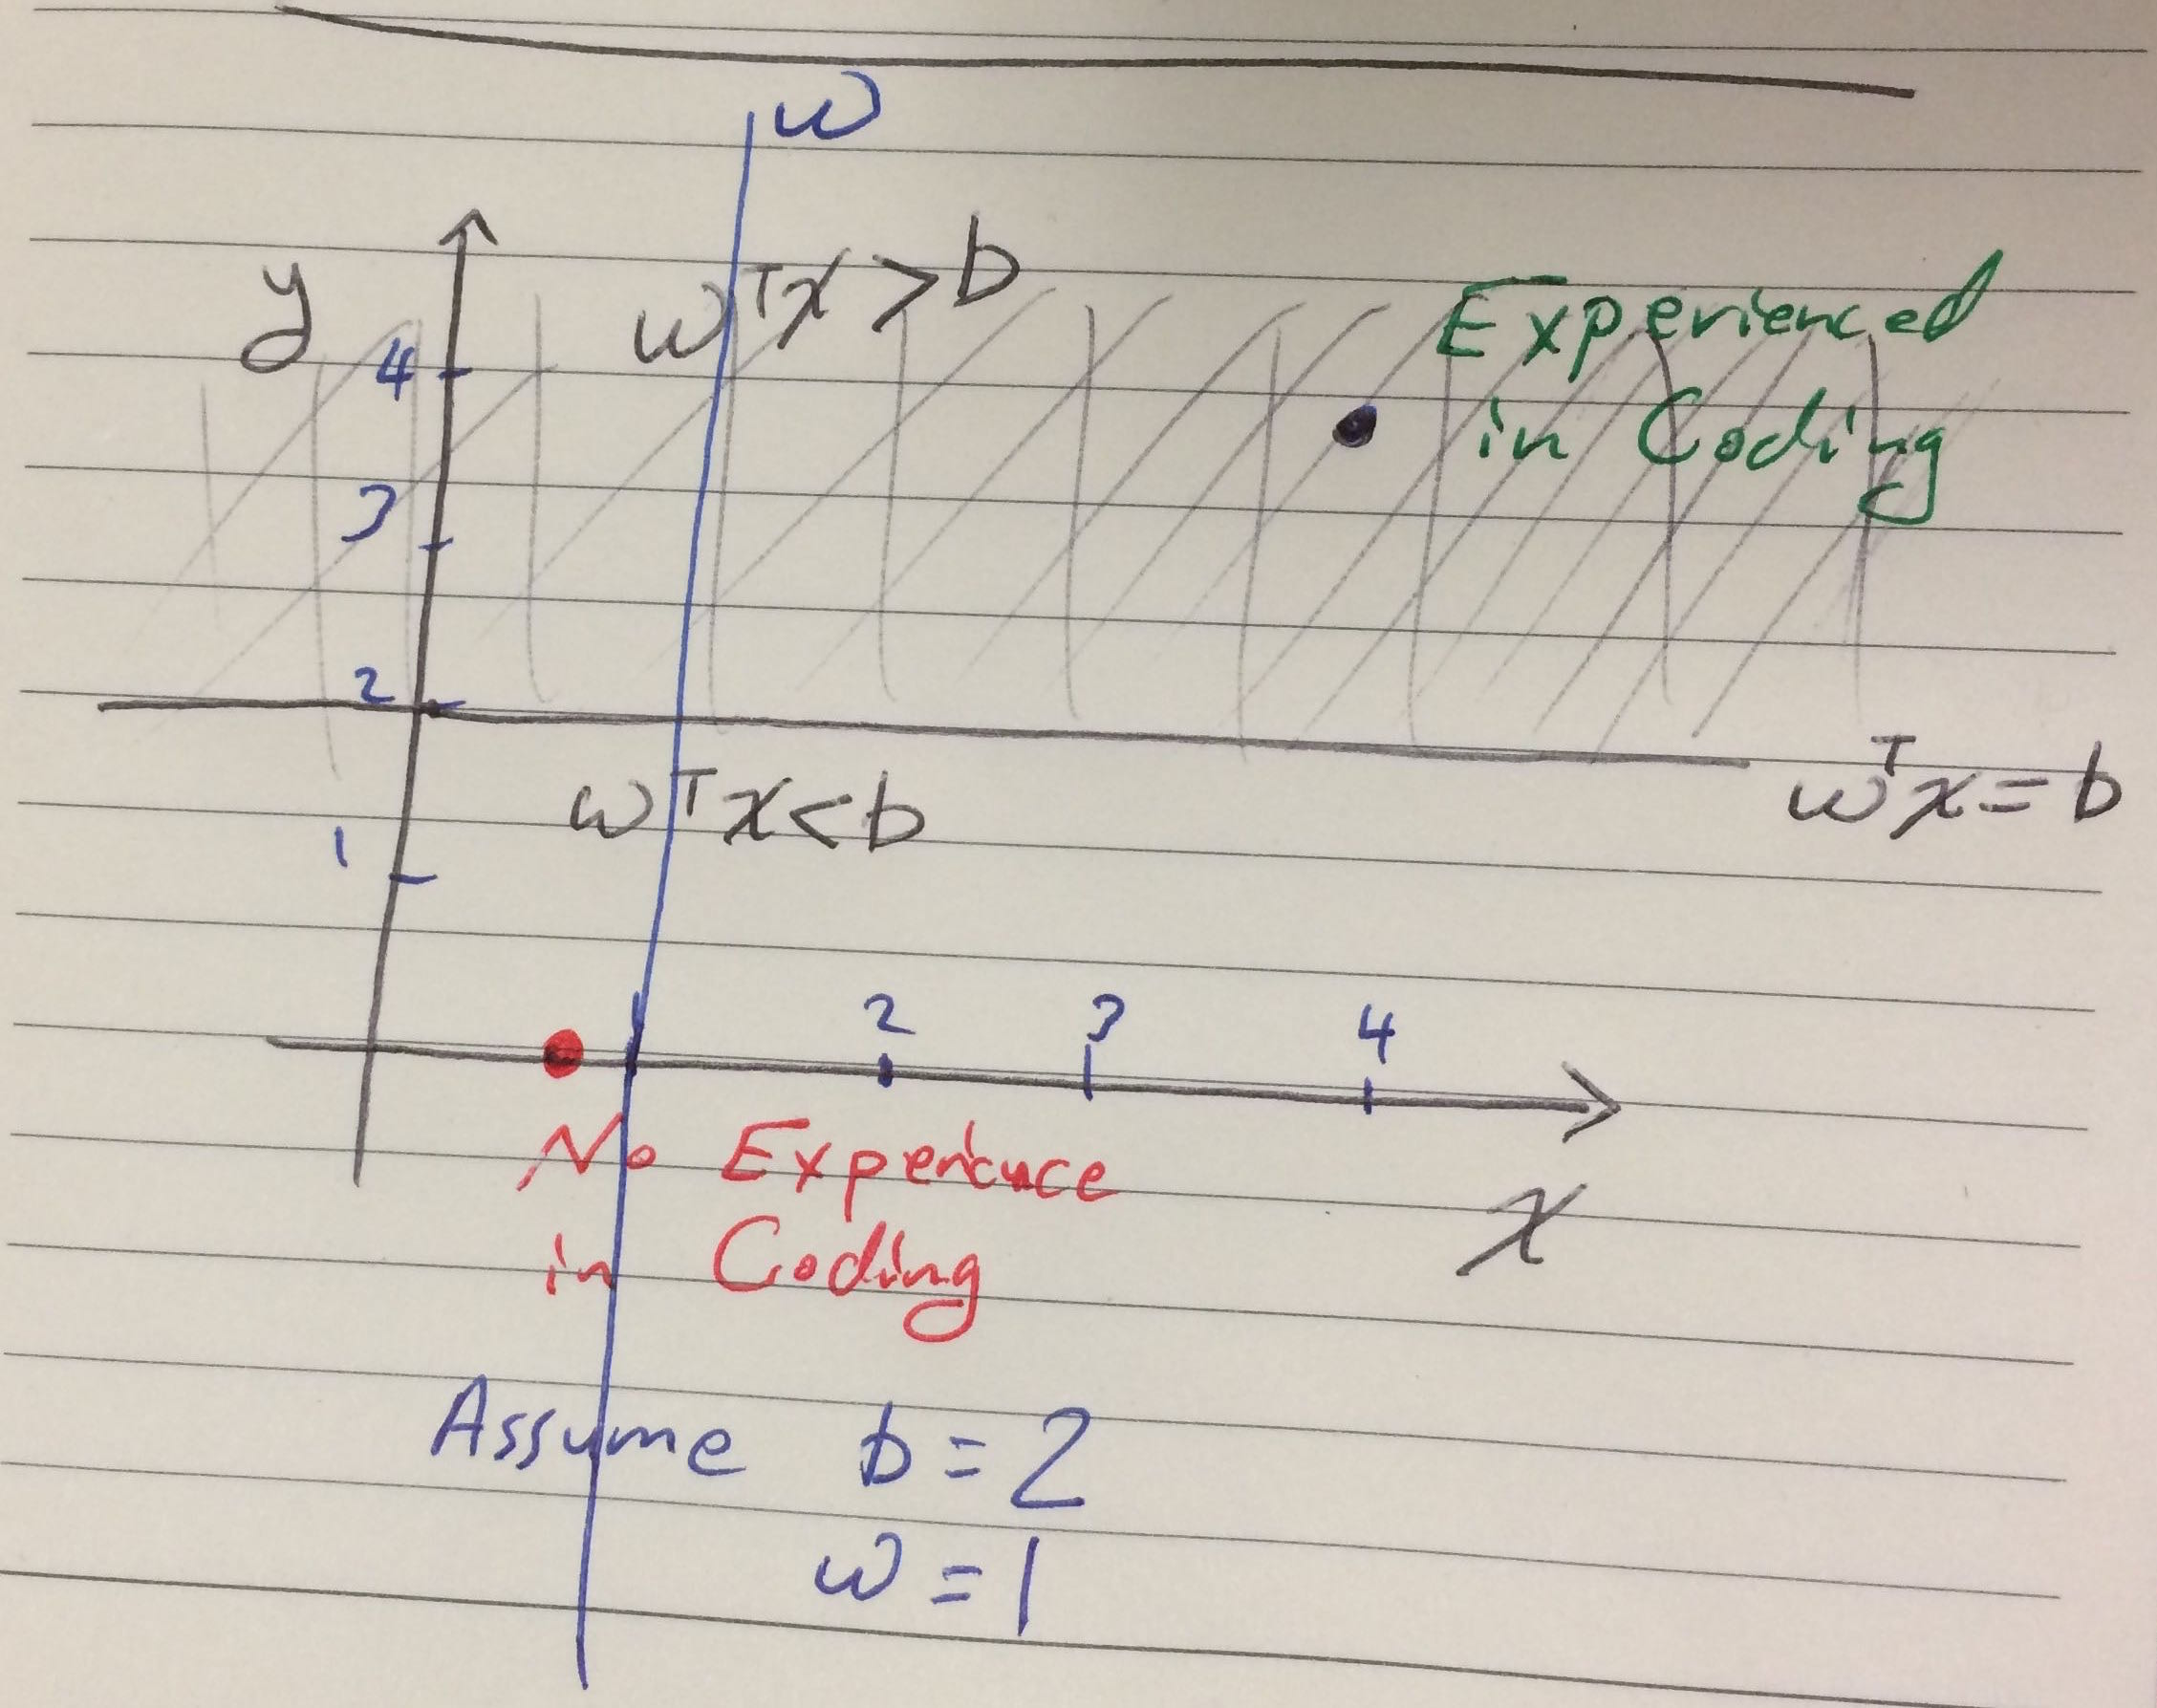
\includegraphics[width=400 pt]{IMG_7313.jpg}
    \caption{Problem 2 parts (i), (ii) and (v) of (e).}
    \label{fig:Mat}
\end{figure}
\section{Problem 2}
\textcolor{red}{\textit{Vectors, matrices and inner products}.}\\

\begin{itemize}
\item After running this: $u = rand(3,1);v = rand(3,1); u'v$ the result is as follows 1*1Array $\lbrace$Float64,2$\rbrace$:
 $0.993625$. On the other hand, running the following $x = rand(3); y = rand(3); x'*y$ provided the following result: $0.91015084477077$. The size of the former result is $(1,1)$ whereas the size of the later result is Epmty! Cearly, Julia distingushes between elements multiplications vs array multiplications. 
\item In the case of using dot vs sum functions for vectors $u$ and $v$, the results are exactly the same, we got a scalar. Likewise, for the case of vectors $x$ and $y$. 
\item The results I got after running A[1,:] vs A[:,1] was, surprisingly, the same. The result is always a 5-element Array. Frankly speaking, I was expecting to get a column vector and a row vectors respectively just like what you get in MATLAB! Clearly, the answer is we get vectors.
\item sum(A[:,1].*A[1,:]) or dot(A[:,1],A[1,:]).
\item .
\item .  
\end{itemize}



\end{document}
